    \subsection*{Linear regression problem}

        \begin{wrapfigure}[18]{r}{0.33\columnwidth}
            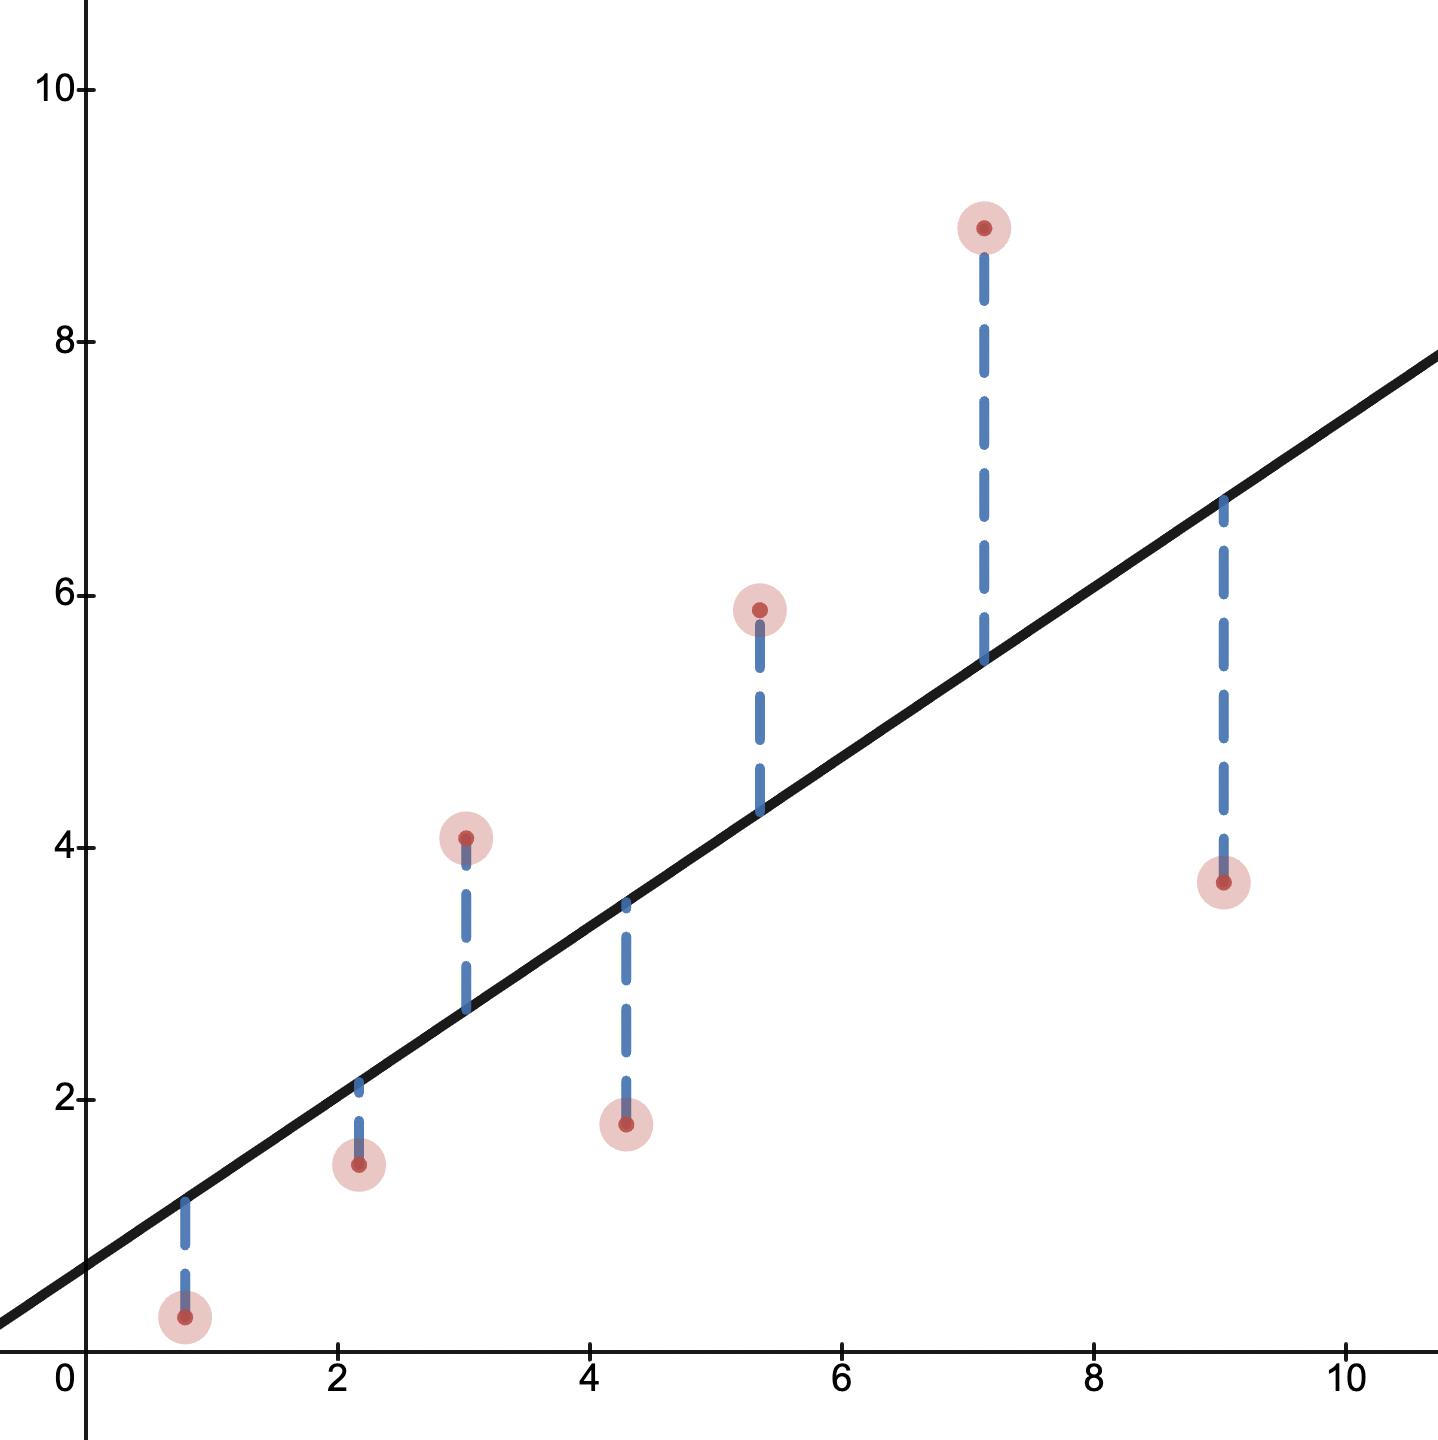
\includegraphics[width=0.33\columnwidth]{lectures/images/linear_regression.png}
            \caption*{\scriptsize{In linear regression, the observations (red) are assumed to be the result of random deviations (blue) from an underlying relationship (black) between a dependent variable (y) and an independent variable (x).}}
            \label{fig:inconsistent_with_vectors}
        \end{wrapfigure}  
        
        Let $y,x_1,x_2,\ldots,x_n$ be variables. We believe that  dependent variable $y$ could be approximated by linear combination of independent variables $x_1,x_2,\ldots,x_n$. That is,
        $$
           y\approx  a_1x_1+a_2x_2+\cdots +a_nx_n .
        $$
        The problem is to find coefficients $a_1,a_2,\ldots,a_n$. In order to find them we conduct $m$ experiments (samples) and get following dataset of observations
        $$
        \begin{cases}
            y_1\approx a_1x_{11}+\ldots+a_nx_{n1} \nonumber\\    
            y_2\approx a_2x_{12}+\ldots+a_nx_{n2} \nonumber\\    ~~~~~~~~~~~~~~~~~~\vdots~~~~~~~~~~~~~~~~~\nonumber\\
            y_m\approx a_1x_{1m}+\ldots+a_nx_{nm} \nonumber
        \end{cases}
        $$ 
        where $x_{1i},x_{2i},\ldots,x_{ni},y_i$ is a result of $i$-th experiment. Clearly, the problem could is equivalent to matrix equation of the form   
        \begin{eqnarray}
            X\vec{a}\approx\vec{y},\nonumber
        \end{eqnarray}
        where 
        $$
            X=
            \begin{bmatrix}
                x_{11} & \cdots & x_{1n}\\
                \vdots & \ddots & \vdots\\
                x_{m1} & \cdots & x_{nm} 
            \end{bmatrix},
            \quad
            \vec{a}=
            \begin{bmatrix}
                a_{1}\\
                \vdots\\
                a_{n}\\
            \end{bmatrix},\quad
            \vec{y}=
            \begin{bmatrix}
                y_{1}\\
                \vdots\\
                y_{m}\\
            \end{bmatrix}.\quad
        $$
        The solution of the problem is least square solution (pseudosolution)
        $$
        \vec{a}=X^+\vec{y}.
        $$

        \begin{problem}{Linear regression}
            Find linear approximation of temperature using following dataset of temperature observations. Find temperature on day $4$.
            \begin{center}
            \begin{tabular}{ |c|c|c| } 
             \hline
             $\#$ & Day & Temperature \\\hline
             1& 1 & 19\textdegree \\ 
             2& 2 & 18\textdegree \\ 
             3& 2 & 20\textdegree \\ 
             4& 3 & 15\textdegree \\ 
             \hline
            \end{tabular}
            \end{center}
            \begin{solution}
                Let us denote day and temperature of the row $i$ by $x_i$ and $y_i$ respectively. We assume that temperature ($y(x)$) could be approximated by linear model 
                $$
                y(x)=ax+b\in\mathbb{R},
                $$
                where $x\in\mathbb{R}$ is number of the day and $a,b\in\mathbb{R}$ are unknown coefficients. This means that we need to find pseudosolution of the following system
                $$
                    X\vec{a}=\vec{y},
                $$
                where
                $$
                    X=
                    \begin{bmatrix}
                        1 & 1 \\
                        2 & 1 \\
                        2 & 1 \\
                        3 & 1 
                    \end{bmatrix},\quad
                    \vec{y}=
                    \begin{bmatrix}
                        19\\
                        18\\
                        20\\
                        15
                    \end{bmatrix},\quad
                    \vec{a}=
                    \begin{bmatrix}
                        a\\
                        b
                    \end{bmatrix}.
                $$
                So we need to evaluate the following $\vec{a}=X^+\vec{y}$. Since $X$ is full column rank, we get 
                \begin{eqnarray}
                    X^+&=&(X^*X)^{-1}X^*
                    =\left(2
                    \begin{bmatrix}
                        9 & 4\\
                        4 & 2
                    \end{bmatrix}
                    \right)^{-1}
                    X^*\nonumber\\
                    &=&
                    \dfrac{1}{2}
                    \dfrac{1}{2}
                    \begin{bmatrix}
                        2 & -4\\
                        -4 & 9
                    \end{bmatrix}
                    \begin{bmatrix}
                        1 & 2 & 2 & 3\\
                        1 & 1 & 1 & 1
                    \end{bmatrix}\nonumber\\
                    &=&
                    \dfrac{1}{4}
                    \begin{bmatrix}
                        -2 & 0 & 0 & 2\\
                        5 & 1 & 1 & -3
                    \end{bmatrix}\nonumber
                \end{eqnarray}
                Hence, we get
                $$
                    \vec{a}=
                    X^+\vec{y}=
                    \dfrac{1}{4}
                    \begin{bmatrix}
                        -2 & 0 & 0 & 2\\
                        5 & 1 & 1 & -3
                    \end{bmatrix} 
                    \begin{bmatrix}
                        19\\
                        18\\
                        20\\
                        15
                    \end{bmatrix}
                    =
                    \begin{bmatrix}
                        -2\\
                        22
                    \end{bmatrix}.
                $$
                This means that linear model $y(x)$ is 
                $$
                    y(x)=-2x+22.
                $$
                According to linear model $y(x)$, on day 4 temperature will be $y(4)=14$\textdegree.
            \end{solution}
        \end{problem}